% Define document class
\documentclass[usenatbib,fleqn,letters]{mnras}
\usepackage{showyourwork}
\usepackage{graphicx}
\usepackage{amssymb,amsmath}
\usepackage{color}
\usepackage{multirow}
\usepackage{soul}
\usepackage{orcidlink}
\usepackage{comment}


\newcommand{\sarc}{$^{\prime\prime}\!\!$}
\newcommand{\myreferences}{references.bib}
\newcommand{\frii}{FR$\,$II}
\newcommand{\fri}{FR$\,$I}
\newcommand{\wphz}{$\,$W$\,$Hz$^{-1}$}
\newcommand{\tbpeak}{$T_{b,\mathrm{peak}}$}
\newcommand{\tbtotal}{$T_{b,\mathrm{total}}$}
\newcommand{\muJybm}{$\mu$Jy$\,$beam$^{-1}$}
\newcommand{\llof}{$L_{\textrm{144MHz}}$}

\defcitealias{morabito_identifying_2022}{M22}
\defcitealias{best_lofar_2023}{B23}

% Title
\title[A hidden AGN population]{A hidden Active Galactic Nuclei population: the first radio luminosity functions constructed by physical process instead of galaxy classification}

% Author list
\author[L.K. Morabito]{\parbox{\textwidth}{Leah K. Morabito$^{1,2}$\thanks{E-mail: leah.k.morabito@durham.ac.uk}\orcidlink{0000-0003-0487-6651}
J.M.G.H.J. de Jong$^{3}$,
F. Sweijen$^{1}$,
R. Kondapally$^{4}$,
P.N. Best$^{4}$,
B. Yue$^{4}$, and friends
\\}\\ 
$^{1}$Centre for Extragalactic Astronomy, Department of Physics, Durham University, Durham DH1 3LE, UK \\
$^{2}$Institute for Computational Cosmology, Department of Physics, Durham University, South Road, Durham DH1 3LE, UK \\ 
$^{3}$Leiden \\
$^{4}$Edinburgh \\}

% Begin!
\begin{document}

\date{}
\pagerange{\pageref{firstpage}--\pageref{lastpage}} \pubyear{2024}
\maketitle

\label{firstpage}


% Abstract with filler text
\begin{abstract}
Both star formation (SF) and Active galactic nuclei (AGN) play an important role in galaxy evolution. Quantifying their relative importance in a statistical way can be done using radio luminosity functions. Until now these have relied on galaxy classifications, with sources which have a mixture of radio emission from SF and AGN assigned to either a star-forming galaxy or an AGN. This can lead to the under-estimation of the relevance of AGN, or an over-estimation of SF. Brightness temperature methods were demonstrated to be effective at 144 MHz using sub-arcsecond imaging with the International LOFAR Telescope (ILT) in \cite{morabito_identifying_2022}. We use the combination of sub-arcsecond and arcsecond resolution imaging of 7,497 sources in the Lockman Hole and ELAIS-N1 fields to identify AGN components in the high resolution images and subtract them from the total flux density, leaving behind flux density from SF only. We construct, for the first time, radio luminosity functions by physical process rather than galaxy classification, revealing a hidden AGN population at \llof $<10^{24}$\wphz . This population is $\sim$50 percent more than expected for $0.5<z<2.0$. The star forming population is less impacted, with only $\sim$10 - 20 percent less star formation than expected. The contribution of `hidden' AGN to the overall radio population, especially at \llof $<10^{24}$\wphz , is significant, and only revealed thanks to the combination of the ILT's resolution and wide field of view. \vspace{3.7in}
\end{abstract}




% Main body with filler text
\section{Introduction}
\label{sec:intro}
The extent to which active galactic nuclei (AGN) impact galaxy formation is a major open question in astrophysics. It is clear that there is an interaction, from both observational and theoretical standpoints. Observations have revealed tight scaling relations between the mass of a super-massive black hole and its host galaxy \citep[see, e.g.][and references therein]{kormendy_coevolution_2013}, while cosmological simulations require some form of AGN feedback \citep{bower_breaking_2006,croton_many_2006} to be able to reproduce the observed galaxy population. 
%Galaxies build up their stellar mass through star formation, while super-massive black holes are expected to provide either negative or positive feedback to either suppress or stimulate galaxy growth, although whether we can definitively pinpoint which type of feedback is an open question \citep{ward_cosmological_2022}. 
The cosmic history of AGN activity and star formation (SF), and by extension the interplay between them, are interlinked. It is necessary to quantify the contribution of each process to understand the importance of either or both of them. Relying on overall galaxy classification can over- or under-estimate the contributions of each process; for example, by considering all of the radio emission in a galaxy classified as `star-forming' to be due to star formation, when some may be due to AGN. Quantifying this is the goal of this letter. 

Decomposing AGN activity from star formation is a difficult problem at any wavelength. Efforts have been made to do this via mid-infrared (MIR) spectral decomposition using template fitting \citep[e.g.,][]{laurent_mid-infrared_2000,hernan-caballero_resolving_2015,li_active_2024}. Multi-wavelength approaches use spectral energy distribution (SED) fitting, which utilises information from a much broader number of observed bands to jointly fit galaxy and AGN components \citep[e.g.][]{calistro_rivera_agnfitter_2016,boquien_cigale_2019,pacifici_art_2022}. However, SED fitting is costly as it relies on observations using many different instruments over the same part of the sky, which then have to be carefully cross-matched. Varying selection effects across the different bands can also present a problem. 

An alternative method to unambiguously identify the AGN component(s) in a galaxy is through brightness temperature, $T_b$, measurements in the radio waveband. Radio emission has the advantage of being unobscured by dust or gas, meaning there are minimal selection effects. %Brightness temperature is a non-physical temperature which is defined as the temperature of a blackbody which would produce the observed surface brightness. 
Models of radio emission from SF predict an upper limit to the surface brightness that can be produced, even in starburst galaxies \citep{condon_radio_1992}. Surface brightness which is detected above this limit therefore has to be attributed to AGN activity. Brightness temperature is inversely proportional to frequency and resolution, $T_b \propto \nu^{-2}\Omega^{-1}$ (where $\Omega \propto \theta_{maj}\theta_{min}$). Traditionally brightness temperature measurements require Very Long Baseline Interferometry (VLBI) which achieve milli-arcsec resolutions at GHz frequencies \citep[e.g.,][]{middelberg_mosaiced_2013,herrera_ruiz_faint_2017,radcliffe_nowhere_2018} to achieve enough sensitivity to make meaningful measurements. In \cite{morabito_identifying_2022} (hereafter, \citetalias{morabito_identifying_2022}) we demonstrated using sub-arcsecond resolution (0.\sarc\ 3) at 144 MHz with the LOw Frequency ARray \citep[LOFAR;][]{van_haarlem_lofar:_2013}. The advantage of LOFAR is its wide field of view: $\sim$6 deg$^2$ from a single observation versus a few to a couple hundred arcmin$^2$ with VLBI at GHz frequencies, depending on whether one is imaging at the phase centre of the observation or using multi-phase centres for correlation \citep{deller_difx-2:_2011,morgan_vlbi_2011}. For example, using an 8 hour LOFAR observation of the Lockman Hole \citep{sweijen_deep_2022} we identified 940 AGN via brightness temperature \citepalias{morabito_identifying_2022}, providing a sample two orders of magnitude larger than any VLBI sample of AGN identified at GHz frequencies. 

As part of the LOFAR Two-metre Sky Survey Deep Fields \citep{sabater_lofar_2021,tasse_lofar_2021} campaign, we have now doubled the areal coverage of 0.\sarc\ 3 resolution wide-field imaging. \cite{de_jong_into_2024} recently published their 0.\sarc\ 3 resolution image of the ELAIS-N1 field, which reaches a depth of 14 $\mu$Jy$\,$bm$^{-1}$ using 32 hours of observations. They also demonstrate the flexible resolution which can be achieved with LOFAR, by imaging at 0.\sarc\ 6 and 1.\sarc\ 2 resolution, which are both complementary to the existing 6\sarc\ \ Deep Fields Data Release 1 (DR1). Again this has an advantage over VLBI with instruments at GHz frequencies, which require either observing at different frequency bands or with other instruments to acquire information on the flux density of sources at other scales. As described in \S~5 of \citepalias{morabito_identifying_2022}, for sources which are unresolved in the 0.\sarc\ 3 resolution images and do not exhibit a radio excess over that predicted the star formation rate (SFR) derived from SED fitting \citep[see][for more details]{best_lofar_2023}, we can separate the AGN activity from SF using a combination of the 0.\sarc\ 3 and 6\sarc\ \ resolution images. 


The 2,483 sources in Lockman Hole \citep{sweijen_deep_2022} and now the 13,058 sources in ELAIS-N1 \citep{de_jong_into_2024}, represents a massive step towards robust statistical studies where the population can be broken into bins of redshift and stellar mass to investigate the AGN and SFG populations in detail. \cite{cochrane_lofar_2023} and \cite{kondapally_cosmic_2022} constructed radio luminosity functions (RLFs) from the 6\sarc\ \ resolution imaging that formed the Deep Fields DR1 for the star forming galaxies and radio-excess AGN, respectively. Here we construct RLFs, for the first time, by process rather than overall galaxy classification. We do this by using a combination of the 0.\sarc\ 3 and 6\sarc\ \ resolution imaging from Lockman Hole and ELAIS-N1. We investigate the cosmic evolution of AGN activity and SF by dividing the sample into redshift bins. 

In this paper, we first describe the data and methods in \S~\ref{sec:data}, followed by an overview of the methods in \S~\ref{sec:methods}. Section~\ref{sec:results} describes the results, followed by 
% discussion and 
conclusions in 
%\S~\ref{sec:discussion} and
\S~\ref{sec:conclusions}
%, respectively
.

Throughout this paper, we use a $H_0 = 70$ km$\,$s$^{-1}\,$Mpc$^{-1}$, $\Omega_M = 0.3$, and $\Omega_{\Lambda}= 0.7$ cosmology. Radio flux density is defined as $S\propto \nu^{\alpha}$ where $\nu$ is frequnecy and $\alpha$ is radio spectral index. 

%Stuff and things \citep{morabito_sub-arcsecond_2022}.

\section{Data}
\label{sec:data}

\subsection{LoTSS Deep Fields DR1}
\label{subsec:dr1}
The LOFAR Two-metre Sky Survey (LoTSS) has both a wide-area \citep{shimwell_lofar_2017,shimwell_lofar_2021,shimwell_lofar_2022} and Deep Fields \citep{tasse_lofar_2021,sabater_lofar_2021} component. The Deep Fields Data Release 1 (DR1) in 2021 included Boötes, Lockman Hole, and ELAI-N1, reaching sensitivities of 30, 23, and 20 \muJybm , using $\sim$80, $\sim$100, and $\sim$160 hours, respectively. The resolution of these images is all 6\sarc . Alongside these deep radio images and their associated catalogues, \cite{kondapally_lofar_2021} provided a careful compilation of the ancillary deep data at other wavebands (from far-infrared to ultraviolet) and cross-matching to the radio catalogues, followed by photometric redshifts and stellar mass estimates in \cite{duncan_lofar_2021}. Collectively these catalogues provide an excellent resource, and we refer the reader for more details to the individual papers cited above.

Based on the cross-matched multi-wavelength catalogue \cite{kondapally_lofar_2021}, \cite{best_lofar_2023} (hereafter, \citetalias{best_lofar_2023}) carried out detailed SED fitting for all radio-detected sources across the three deep fields, using the multi-wavelength data. Full details can be found in their paper, but here we outline the relevant details. All sources detected above 5$\sigma$ in their respective radio images had their far-infrared (FIR) to ultraviolet (UV) data fit using four different SED fitting software packages. These were: MAGPHYS \citep{da_cunha_simple_2008}, BAGPIPES \citep{carnall_inferring_2018,carnall_how_2019}, CIGALE \citep{burgarella_star_2005,noll_analysis_2009,boquien_cigale_2019}, and AGN\textsc{fitter} \citep{calistro_rivera_agnfitter_2016}. The first two (MAGPHYS and BAGPIPES) use an energy balance approach, where optical to UV energy absorbed by dust must be transferred to thermal emission in the FIR to sub-mm.  CIGALE also uses the same energy-balance approach, but includes an AGN component. The final code, AGN\textsc{fitter} is designed to work in cases where the UV light and IR emission are spatially distinct, and thus the energy balance assumption does not hold. Many AGN fall under this umbrella. Each galaxy was fit with all four codes (twice for CIGALE, using different AGN components) and a `consensus' value found for the derived galaxy properties using information from the goodness-of-fits.  

The derived properties used in this paper are the consensus SFRs, and the galaxy classifications which arise from the SED fitting. \citetalias{best_lofar_2023} use the relationship between radio luminosity and SFR to define sources as either \textit{radio excess} or not, based on the expected relationship between radio luminosity and SFR. The AGN components used to fit the multi-wavelength information indicate whether a source is a radiatively efficient AGN (i.e., is there evidence for a disk/torus structure) or not. Combining these provides the following classes:
\begin{itemize}
    \item Radio excess + radiatively efficient (\textit{`radio-loud'})
    \item Radio excess + not radiatively efficient (\textit{`radio-loud'})
    \item Radiatively efficient + not radio excess (\textit{`radio-quiet'})
    \item Radiatively inefficient + not radio excess
\end{itemize}
The first three classes are AGN, and the final class is star forming galaxies (SFGs).  Five percent of all sources are Unclassified, as they do not have a radio excess and the fits could not determine between radiatively efficient or inefficient. 


\subsection{High-resolution LOFAR imaging}
\label{subsec:highres}

Data for LoTSS is recorded with all available LOFAR stations, which are spread across nine different European countries, with a preponderance of stations in the Netherlands. The longest baseline (currently Ireland to Latvia) is $\sim$2,000 km, providing unprecedented resolution at MHz frequencies. While LoTSS uses only the stations in the Netherlands for its standard data processing, post-processing of LoTSS data to achieve sub-arcsecond resolution is ongoing both for individual sources with $S>10\,$mJy in the wide-area survey \citep{morabito_sub-arcsecond_2022} and for the entire field of view in the Deep Fields \citep[][Escott et al., in prep; Bondi et al., in prep]{sweijen_deep_2022,de_jong_into_2024}. %While the full field of view imaging is currently too computationally expensive for the wide area, we are focusing on the Deep Fields. 
Due to the fact that the station layout of international stations is larger than that of stations in the Netherlands, the station beams have a smaller field of view. Coupled with bandwidth and time smearing, this limits the field of view effectively to a radius of 1.24 deg, which still provides 6.25 deg$^2$ of coverage\footnote{The imaged field of view is square with 2.5 deg per side.}. 

Both Lockman Hole and ELAIS-N1 have been imaged at 0.\sarc\ 3 resolution \citep[][respectively]{sweijen_deep_2022,de_jong_into_2024}. The resulting images have median rms noise of 34 \muJybm\ (Lockman Hole) and 14 \muJybm\ (ELAIS-N1), although the noise is lowest in the centre and increases radially in both images. Catalogues from these images were processed to group individual Gaussian islands into complete sources, and remove duplicates. The resulting catalogues contain 2,316 and 13,058 sources above 5$\sigma$, for Lockman Hole and ELAIS-N1 respectively. Although \cite{de_jong_into_2024} also imaged ELAIS-N1 at 0.\sarc\ 6 and 1.\sarc\ 2, for consistency with Lockman Hole we use only the 0.\sarc\ 3 and 6\sarc\ resolution images. 

%The Lockman Hole was the first field to have its full field of view imaged at 0.\sarc\ 3 resolution \citep{sweijen_deep_2022}. This took a quarter million cpu hours to produce a single 7-billion pixel image from 8 hours of data. 
%The resulting image has a median rms noise of 34 \muJybm , although this is lower in the centre and higher in the outskirts. From this image, a catalogue of 2,316 5$\sigma$ sources was created, removing duplicates and grouping individual Gaussian islands together into sources. 
%The first 0.\sarc\ 3 image of ELAIS-N1 was recently published \citep{de_jong_into_2024}, along with companion images at intermediate resolutions of 0.\sarc\ 6 and 1.2\sarc . The median rms noise reaches 14 \muJybm\ in the centre of the 0.\sarc\ 3 resolution image, and increases radially. For consistency with the Lockman Hole sample, we do not use the intermediate resolution images here. In the 0.\sarc\ 3 resolution image, there were 13,058 sources catalogued above 5$\sigma$ after grouping Gaussian islands into sources and removing duplicates. 

Thanks to the added collecting area of the international stations, which increases the sensitivity of the array, the 0.\sarc\ 3 resolution image for ELAIS-N1 is \textit{deeper} than the Deep Fields DR1. To ensure consistently built samples, and make use of DR1 information, we limit the high-resolution catalogues. For both fields, 
%The derived galaxy properties from \citetalias{best_lofar_2023} (see \S~\ref{subsec:dr1}) were for LoTSS Deep Fields DR1, and thus we have to limit the source catalogues we wish to use. For both Lockman Hole and ELAIS-N1 catalogues derived from the 0.\sarc\ 3 resolution images, 
we first find the local rms in the companion 6\sarc\ \ resolution noise maps\footnote{\label{dr1}Available at \href{https://lofar-surveys.org/deepfields.html}{https://lofar-surveys.org/deepfields.html}} at the position of each source in the 0.\sarc\ 3 resolution catalogue. Using the peak brightness of the source in the catalogue from the 0.\sarc\ 3 resolution image, we calculate the peak-to-noise ratio and only select sources which would be detectable at the 5$\sigma$ limit in the 6\sarc\ resolution image, effectively ensuring all sources will have a match in DR1. We then cross-match based on radio position, to provide the radio information from the catalogues derived from both the 0.\sarc\ 3 resolution image and the 6\sarc\ \ resolution image. We trim the area down for each field using their respective optical starmasks\textsuperscript{\ref{dr1}} by selecting sources which are not contained in the null areas of these masks. This removes sources where the multi-wavelength information is impacted by bright stars. Finally, we trim the area down to the 2.5 deg$\times$2.5 deg area which is covered by the 0.\sarc\ 3 resolution image. We are left with \variable{output/lockman_detectable.txt}sources in Lockman Hole, and \variable{output/en1_detectable.txt}sources in ELAIS-N1. We use the source name from the catalogue derived from the 6\sarc\ \ resolution to cross-match to the catalogue from \citetalias{best_lofar_2023}. 

We determine whether sources are resolved or unresolved in the same manner as \S~3.1 of \cite{shimwell_lofar_2019,shimwell_lofar_2022}. Truly unresolved sources in radio maps should have equal peak brightness and integrated flux density, but LOFAR maps are impacted by smearing due to the ionosphere. This causes resolved sources to have a lower peak brightness when compared to the integrated flux density, and they can appear spatially extended. We start by selecting sources which are fit by a single Guassian component ({\ttfamily S\_CODE = `S'}), and make a cut to remove sources which are larger than a multiple of the beam size. For the Lockman Hole, we use a factor of 3, but for ELAIS-N1 we find that a factor of 4 provided a better sample. This may be because half of the data for ELAIS-N1 had been pre-averaged to 2 sec integration times, which will increase the time smearing \citep[see \S~2 in][]{de_jong_into_2024}. We fit a Sigmoid function to find the upper 99.9th percentile of sources considering their integrated flux density to peak brightness ratio as a function of the local signal to noise. Anything above this boundary is considered to be resolved. We also treat sources which do not have {\ttfamily S\_CODE = `S'} as resolved.

\begin{comment}
\subsection{Simulations}
\label{subsec:simba}

We use the SIMBA cosmological hydrodynamic simulation which accounts for an H$_{2}$ based star formation rate following the sub-grid model of \cite{krumholz_comparison_2011}. Additionally, SIMBA models the growth of supermassive black holes via a two-mode prescription based on the temperature of gas within a distance, $R_{0}$, calculated over the 256 nearest particles limited to 2$h^{-1}$kpc. 
It is commonplace for cosmological simulations to employ the growth of SMBHs via the Bondi rate \hl{citations EAGLE, HORIZON AGN, Illustris, TNG}. In SIMBA, the Bondi rate is employed when gas within $R_{0}$ has temperatures T$>10^{5}$K, referred to as the hot mode. What makes SIMBA unique is the additional contribution to the accretion rate via a torque limited accretion flow when gas has temperatures T$<10^{5}$K, or in the cold mode. 
SIMBA also employs a physically motivated model for AGN feedback in the form of AGN winds \citep{perna_x-raysdss_2017}, as well as AGN jets with velocities that increase inversely proportional to the Eddington rate in accordance with \cite{heckman_coevolution_2014}.
SIMBA therefore provides a platform to study jet-mode AGN in a way that has not been explored before. 
Specifically, we select galaxies in SIMBA that have full-velocity jets, that is, when the Eddington rate drops below 0.02 (but non-zero) and where the black hole mass is larger than M$_{\rm BH}>10^{8}$M$_{\odot}$. For this population we are able to calculate the amount of radio emission due to star formation processes following \cite{condon_radio_1992} as well as that from accretion processes following \cite{kording_measuring_2008}. Details of this method can be found in \cite{thomas_radio_2021}. We can therefore calculate the contribution to the radio luminosity function from star formation and AGN accretion processes. We can additionally separate the galaxy population into star forming and quiescent galaxies, radio-excess, or radiatively efficient and inefficient, based on the sources black hole and host properties.
\end{comment}

\section{Methods}
\label{sec:methods}

Brightness temperature, $T_b$, is used to characterise the surface brightness of radio emission. It is not a physical temperature, but rather the temperature of a black body  which would produce the observed spectral radiance (assuming the Rayleigh-Jeans approximation) at long wavelengths. By creating a model which predicts the upper limit of $T_b$ achievable by star formation \citep[based on][]{condon_radio_1992}, if the value is \textit{above} that upper limit, the radio emission must be due to AGN activity.  \citetalias{morabito_identifying_2022} showed that this AGN identification can be done at 150 MHz using sub-arcsecond resolution; 
%this works because $T_b\propto\nu^{-2}\Omega^{-1}$ where $\nu$ is the observed frequency and $\Omega$ is the solid angle of the emitting region -- for unresolved sources, this corresponds to the deconvolved beam size. 
we refer the reader to \S~3 of \citetalias{morabito_identifying_2022} for more details. Note that this method yields conservative, positive AGN identifications. There may be lower surface brightness AGN emission which is not identified, and it is also possible \citep[although unlikely, according to][]{condon_radio_1992} that extreme, compact nuclear starbursts could produce AGN-like values of $T_b$. 

\subsection{Separation of AGN activity and SF}
Once the AGN activity is identified from the 0.\sarc\ 3 resolution images, it is possible to separate it from star formation using the total flux density from the 6\sarc\ \ resolution images. We refer the reader to \S~5 in \citetalias{morabito_identifying_2022} for more details but outline the process here, which is depicted in Fig.~\ref{fig:flowchart}. Sources which are identified as radio excess according to the definition in \citetalias{best_lofar_2023} automatically have their total flux density from the 6\sarc\ resolution images added to the AGN category. For sources that are not radio excess, we attribute the total flux density from the 6\sarc\ resolution images to SF if in the 0.\sarc\ 3 resolution image they are either resolved or have no detection. Sources which do not meet these criteria are checked and if their $T_b$ is not above the limit for SF their 6\sarc\ resolution total flux density is also added to the SF category. The total flux density of any source in the 0.\sarc\ 3 resolution image which is $T_b$-identified as an AGN is assumed to be AGN flux density; this is subtracted from the total flux density measured from the 6\sarc\ \ resolution image, and what remains is assumed to be flux density from SF. \variable{output/flowchart_numbers.txt}

\begin{figure}
    \centering
    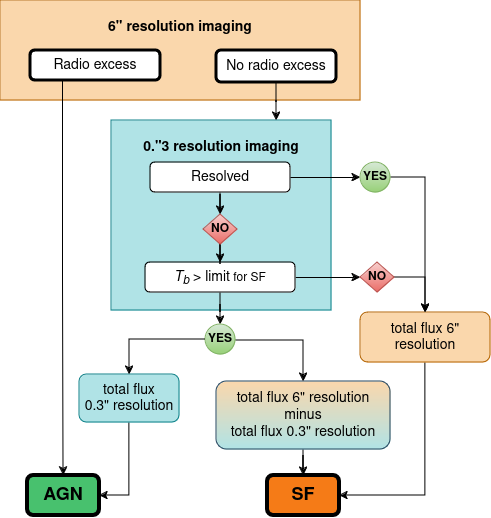
\includegraphics[width=0.5\textwidth]{figures/agn_sf_separation_workflow.png}
    \caption{The workflow for determining how to assign flux density from the 6\sarc\ and 0.\sarc\ 3 resolution images to either the AGN or SF category. Only sources with a $T_b$ identified AGN component have their flux density split between the two categories.}
    \label{fig:flowchart}
\end{figure}

\subsection{Construction of RLFs}

We follow the same method of constructing RLFs as in \cite{kondapally_cosmic_2022} and \cite{cochrane_lofar_2023}. The 0.\sarc\ 3 resolution image is smaller than the 6\sarc\ resolution image, so we first reproduce the published RLFs (Fig.~\ref{fig:rlfs}, left panel) using the galaxy classifications from \citetalias{best_lofar_2023} to check that we have implemented the method appropriately, and that the smaller area yields the same results. We use the completeness corrections from the respective papers. The only correction we do not implement is the photo-$z$ correction used in \cite{cochrane_lofar_2023}. The authors note that this correction is negligible, and as it is not implemented in \cite{kondapally_cosmic_2022} we chose to keep the method for RLF construction in this paper consistent across both samples. We use the same redshift range, $0.003 < z < 0.3$, to verify that we have good agreement with the published RLFs.

Next we use the same method for constructing RLFs by physical process rather than overall galaxy classification. We again use the completeness corrections from \cite{cochrane_lofar_2023} and \cite{kondapally_cosmic_2022}. The completeness corrections are flux density dependent, and we use the overall total flux density of a galaxy, rather than the flux density of the process, which will be smaller if the radio emission from SF and AGN have been split. We still use the overall galaxy completeness correction because this is based on whether or not a \textit{source} will be detectable given the background rms. This only relies on the total flux density, not the flux density of individual components. Even when considering only the SF (or AGN) radio emission in a source, its overall detectability is still derived from the combination of all radio emission processes present. These RLFs for the physical processes of SF and AGN are shown in the middle panel of Fig.~\ref{fig:rlfs}, again for  $0.003 < z < 0.3$. 

% Finally, we use RLFs constructed from SIMBA. The RLFs are constructed as in \cite{thomson_radio_2019}, but have been updated to use the same redshift bins \hl{Nicole}. 

\begin{figure*}
    \centering
    \includegraphics[width=0.98\textwidth]{figures/deep_fields_RLFs.png}
    \caption{\textit{Left:} Validation of our re-calculated galaxy RLFs (dotted lines) for the smaller area considered here with the previously published RLFs (solid lines). \textit{Middle:} RLFs calculated by process rather than galaxy. \textit{Right top:} RLFs calculated here by galaxy classifications (dotted lines) and by physical process (solid lines; orange for AGN and green for SF). \textit{Bottom right:} $\Delta$RLF for both AGN and star formation. }
    \label{fig:rlfs}
    \script{comparison_plot.py}
\end{figure*}


\section{Results}
\label{sec:results}

We present the very first RLFs constructed by physical process rather than galaxy classification. Comparing these with our reproduction of the previously published RLFs, using galaxy classifications, allows us to explore where we are over- or under-predicting the contribution of the physical processes to our statistical studies. To aid this comparison, we define and calculate: 
\begin{equation}
\Delta\textrm{RLF} = \frac{\textrm{RLF(physical process)}}{\textrm{RLF(galaxy classification)}}. \notag
\end{equation}
The $\Delta$RLF is calculated once for the SF category/SFG classification, and once for the AGN category/AGN classification. We show $\Delta$RLF in the bottom right hand panel in Fig.~\ref{fig:rlfs}. We see that above 10$^{24}\,$\wphz\ the ratio for AGN is unity, which is expected where radio excess sources dominate the population. Below that, the ratio for AGN climbs up to $\sim$1.3 and finally almost up to 2 at the lowest radio powers probed. The ratio for SF is always below unity, but it does not deviate as much as the ratio for AGN. This is because the SF population has larger source counts, so the total impact of moving some flux density from the SF to AGN population is less extreme. 

To show the integrated effect of $\Delta$RLF, we integrate each RLF separately across the luminosity bins where both RLFs are defined, and then take the ratio of the areas. For example, for star formation we integrate the RLF for the SF process and the RLF for SFGs, and divide the first by the second. These numbers are always less than unity since the SF process is over-estimated in the SFG population, and this has been corrected by moving $T_b$-identified AGN flux density contributions to the AGN process RLF. These are reported in Tab.~\ref{tab:intvalues}, and show that while the SF process  only decreases by $\sim$10 percent in the lowest redshift bin, the AGN contribution increases by almost a factor of 2. It is evident from the bottom right panel of Fig.~\ref{fig:rlfs} that this `hidden' AGN population extracted from SFGs shows up in the radio AGN population at $L_{\textrm{144MHz}} < 10^{24}\,$\wphz .

\variable{output/integrated_differences.txt}

In Fig.~\ref{fig:evolution} we show the redshift evolution for star formation (left) and AGN (right).  We use similar redshift bins to \cite{kondapally_cosmic_2022} and \cite{cochrane_lofar_2023} for consistency. Some bins become unconstrained for the RLFs by process due to the shuffling of sources between the SF and AGN populations, yielding positve y-axis values. We remove these by cutting out bins where there are more than 4 dex difference between the overall RLF and the process RLF. For the SF RLF we additionally remove points $>1.8$. We reproduce previous observational results that while the SF population has a strong redshift evolution, the AGN population does not. 
%For the simulations, the behaviour is qualitatively similar, although the AGN population does have mild redshift evolution whereas the observations do not.

The bottom panels in Fig~\ref{fig:evolution} show $\Delta$RLF, the same as in the bottom right hand panel of Fig~\ref{fig:rlfs}. For the SF population, $\Delta$RLF is close to unity for $L_{\textrm{144MHz}} < 10^{24}\,$\wphz in the lowest redshift bin, and then this begins to drop at higher luminosities. The higher redshift bins show similar behaviour, perhaps reaching unity at increasingly higher values of $L_{\textrm{144MHz}}$, although deeper data is needed to confirm this. The lowest values reached are $\sim$50 percent. 
%Comparing these ratios between observations and simulations, we see qualitatively the same behaviour, although the simulations reach much lower and higher values for both the SF and AGN populations, respectively. Looking first at the SF population (left set of panels), in the lowest redshift bin the ratio for the simulation stabilises to around unity for \llof $<10^{23}\,$\wphz , and decreases rapidly above this, reaching much smaller values than the observations. Higher redshift bins probe successively higher luminosity ranges, also reaching small values for the ratio between activity and galaxies. This is consistent with the fact that at higher redshifts, most radio AGN in SIMBA are hosted in SFGs, and thus the \textit{galaxy} RLF for SIMBA SFGs is inflated with AGN emission; this makes the ratio of SF activity to galaxy approach zero. 

For the AGN population, $\Delta$RLF has almost the opposite behaviour, converging to unity \textit{above} $\sim$\llof $10^{24}\,$\wphz\ for the lowest redshift bin. This is driven by the fact that the flux density of radio excess sources is entirely attributed to AGN, and these sources tend to have higher radio luminosities. The convergence happens at higher luminosity values for higher redshifts. Below this convergence, across all redshift bins, $\Delta$RLF increases. The maximum value for each redshift bin approaches $\sim$2, although the fact that in the lowest redshift bin the value stabilises at $\sim1.3$ and only climbs higher at the very lowest luminosities (\llof $<10^{22}\,$\wphz ) may be due to incompleteness. If we disregard the lowest luminosity bins, it seems that we see approximately a 30 - 50 percent increase in AGN activity over what is measured when using galaxy classifications alone, for all redshifts. This is borne out by the values in the bottom line of Tab.~\ref{tab:intvalues}, where the difference in the integrated RLFs shows an excess of AGN contribution of $\sim$ 50 percent for the three middle redshift bins. 
%The ratio for the SIMBA RLFs shows strong redshift evolution, and much higher ratio values. The RLFs themselves turn over, whereas the observed RLFs do not. This is likely a consequence of the fact that the AGN emission in SIMBA is due to high-velocity jets, whereas there is increasing observational evidence for low-luminosity jets or AGN emission \citep{macfarlane_radio_2021,yue_novel_2024}. The high values reached by the ratio of RLFs again is expected as many high-$z$ radio AGN in SIMBA are hosted in SFGs. Shifting this AGN emission to AGN \textit{activity} when it is counted in the SFG \textit{galaxy} population generates high values for the activity to galaxy ratio. 
%- sfrd, kinetic LF

\begin{figure*}
    \centering
    \includegraphics[width=\textwidth]{figures/RLF_evolution.png}
    \caption{The redshift evolution of the RLFs (top panels) and $\Delta$RLF (bottom panels) for SF (left) and AGN (right). The dashed horizontal line in the bottom panels is unity, with thin solid horizontal lines at 0.5 (left) at 2.0 (right) to guide the eye.  }
    \label{fig:evolution}
    \script{RLF_evolution.py}
\end{figure*}


\section{Conclusions}
\label{sec:conclusions}

In this letter we have presented, for the first time, RLFs constructed by separating radio emission into either SF or AGN processes, for 7,497 sources. We use brightness temperature to identify AGN components in galaxies with no radio excess, and separate the radio emission for AGN and SF. We compare these with classical RLFs constructed using overall galaxy classifications, and find a hidden AGN population in sources with \llof $\lesssim 10^{24}$\wphz . The integrated impact of this is approximately a 50 percent increase in AGN activity across intermediate redshifts ($0.5 < z < 2.0$), and a doubling in the lowest redshift bin ($0.003 < z < 0.3$). The impact on the star forming galaxy population is less severe, as this population is much larger, amounting to an integrated decrease in the RLF of $\sim$10-20 percent. 

This study is only now possible thanks to LOFAR's exceptional combination of resolution and field of view. The sub-arcsecond resolution is sufficient for brightness temperature identification of AGN, and the field of view means that we have been able to do this for 1,022 sources. We have used conservative limits for AGN identification, which means that there is likely more AGN emission still remaining `uncounted' here. Future work to build a forward modelling method, that can also make use of the intermediate (0.\sarc\ 6 and 1.\sarc\ 2) resolution images will improve the AGN and SF separation. Splitting radio emission into category by physical process also opens up a pathway for more direct comparison to cosmological simulations, which we will address in a future paper.

\vspace{-0.5in}

\section*{Data Availability}
All data used in this paper is either publicly available on \href{https://lofar-surveys.org}{https://lofar-surveys.org} or from the relevant publications cited herein. We have prepared this manuscript using using the showyourwork\footnote{ \href{https://github.com/rodluger/showyourwork}{https://github.com/rodluger/showyourwork}} open source scientific article workflow, which was first introduced in \cite{luger_mapping_2021}. This ensures complete transparency. The code is available at \hl{update link when ready to publish}. 

\section*{Acknowledgements}
LKM is grateful for support from UKRI [MR/T042842/1]. 

LOFAR is the Low Frequency Array designed and constructed by ASTRON. It has observing, data processing, and data storage facilities in several countries, which are owned by various parties (each with their own funding sources), and which are collectively operated by the ILT foundation under a joint scientific policy. The ILT resources have benefited from the following recent major funding sources: CNRS-INSU, Observatoire de Paris and Université d'Orléans, France; BMBF, MIWF-NRW, MPG, Germany; Science Foundation Ireland (SFI), Department of Business, Enterprise and Innovation (DBEI), Ireland; NWO, The Netherlands; The Science and Technology Facilities Council, UK; Ministry of Science and Higher Education, Poland; The Istituto Nazionale di Astrofisica (INAF), Italy. This research made use of the Dutch national e-infrastructure with support of the SURF Cooperative (e-infra 180169) and the LOFAR e-infra group. The Jülich LOFAR Long Term Archive and the German LOFAR network are both coordinated and operated by the Jülich Supercomputing Centre (JSC), and computing resources on the supercomputer JUWELS at JSC were provided by the Gauss Centre for Supercomputing e.V. (grant CHTB00) through the John von Neumann Institute for Computing (NIC). This research made use of the University of Hertfordshire high-performance computing facility and the LOFAR-UK computing facility located at the University of Hertfordshire and supported by STFC [ST/P000096/1], and of the Italian LOFAR IT computing infrastructure supported and operated by INAF, and by the Physics Department of Turin university (under an agreement with Consorzio Interuniversitario per la Fisica Spaziale) at the C3S Supercomputing Centre, Italy.


\begin{comment}
\section*{Appendix A}

\begin{figure*}
    \includegraphics[width=0.49\textwidth]{figures/Lockman_Unresolved_03.png}
    \hfill
    \includegraphics[width=0.49\textwidth]{figures/ELAIS_Unresolved_03.png}
    \caption{\label{fig:unres}The data and sigmoid fits to determine whether sources are resolved or unresolved as described in \S~\ref{subsec:highres}. The \textit{left} panel shows Lockman Hole, and the \textit{right} panel shows ELAIS-N1. }
\end{figure*}

Figure~\ref{fig:unres} shows the integrated flux density to peak brightness ratio as a function of the local signal to noise, parameterised by $\frac{S_{peak}}{2\sigma_{peak}} + \frac{S_{int}}{2\sigma_{int}}$. The data is first binned evenly in log space, and the 99.9th percentile is found in each bin. We then fit a sigmoid function:
\begin{equation}
y = A + \frac{B}{1 + (x / 96.57)^C}, 
\end{equation}
where 96.57 is a fixed value that has worked well for LoTSS \citep{shimwell_lofar_2022}. For Lockman Hole, we find 
\end{comment}

%\clearpage
%\pagebreak


\bibliographystyle{mnras}
\bibliography{references}


\label{lastpage}

\end{document}
